\definecolor{lavander}{cmyk}{0,0.48,0,0}
\definecolor{violet}{cmyk}{0.79,0.88,0,0}
\definecolor{burntorange}{cmyk}{0,0.52,1,0}

\def\lav{lavander!90}
\def\oran{orange!30}

\tikzstyle{time}=[draw,circle,violet,bottom color=\lav,
                  top color= white, text=violet,minimum width=20pt]
                  
\tikzstyle{base}=[draw,circle,burntorange, left color=\oran,
                       text=violet,minimum width=20pt]

\begin{figure}[h!]
\centering
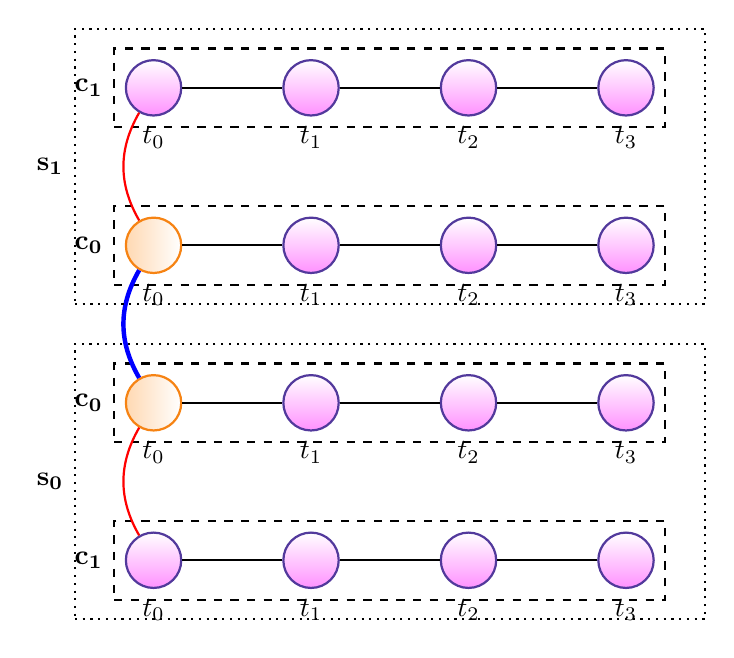
\begin{tikzpicture}[auto, thick]
  % scenario 0
  \node[base,label=below:$t_0$] (s0c0t0) at (0,2) {};
  \node[time,label=below:$t_1$] (s0c0t1) at (2,2) {};
  \node[time,label=below:$t_2$] (s0c0t2) at (4,2) {};
  \node[time,label=below:$t_3$] (s0c0t3) at (6,2) {};
  
  \path (s0c0t0) edge (s0c0t1);
  \path (s0c0t1) edge (s0c0t2);
  \path (s0c0t2) edge (s0c0t3);
  
  % contingency rectangle from (-0.5,1.5) to (6.5,2.5)
   \node[draw,rectangle,dashed,minimum width=7cm,minimum height=1cm,label=left:{$\mathbf{c_0}$}] (s0) at (3.0,2.0) {};
  
  \node[time,label=below:$t_0$] (s0c1t0) at (0,0) {};
  \node[time,label=below:$t_1$] (s0c1t1) at (2,0) {};
  \node[time,label=below:$t_2$] (s0c1t2) at (4,0) {};
  \node[time,label=below:$t_3$] (s0c1t3) at (6,0) {};
  
  \path (s0c1t0) edge (s0c1t1);
  \path (s0c1t1) edge (s0c1t2);
  \path (s0c1t2) edge (s0c1t3);
  
  % contingency rectangle from (-0.5,-0.5) to (6.5,0.5)
   \node[draw,rectangle,dashed,minimum width=7cm,minimum height=1cm,label=left:{$\mathbf{c_1}$}] (s0) at (3.0,0.0) {};
  
   \path (s0c0t0) edge [bend right,color=red] (s0c1t0);
  
  % scenario rectangle from (-1.0,-0.75) to (7.0,2.75)
   \node[draw,rectangle,dotted,minimum width=8cm,minimum height=3.5cm,label=left:{$\mathbf{s_0}$}] (s0) at (3.0,1.0) {}; 
  
  % scenario 1
  \node[base,label=below:$t_0$] (s1c0t0) at (0,4) {};
  \node[time,label=below:$t_1$] (s1c0t1) at (2,4) {};
  \node[time,label=below:$t_2$] (s1c0t2) at (4,4) {};
  \node[time,label=below:$t_3$] (s1c0t3) at (6,4) {};
  
  \path (s1c0t0) edge (s1c0t1);
  \path (s1c0t1) edge (s1c0t2);
  \path (s1c0t2) edge (s1c0t3);
  
   % contingency rectangle from (-0.5,3.5) to (6.5,4.5)
   \node[draw,rectangle,dashed,minimum width=7cm,minimum height=1cm,label=left:{$\mathbf{c_0}$}] (s0) at (3.0,4.0) {};
  
  \node[time,label=below:$t_0$] (s1c1t0) at (0,6) {};
  \node[time,label=below:$t_1$] (s1c1t1) at (2,6) {};
  \node[time,label=below:$t_2$] (s1c1t2) at (4,6) {};
  \node[time,label=below:$t_3$] (s1c1t3) at (6,6) {};
  
  \path (s1c1t0) edge (s1c1t1);
  \path (s1c1t1) edge (s1c1t2);
  \path (s1c1t2) edge (s1c1t3);
  
   % contingency rectangle from (-0.5,5.5) to (6.5,6.5)
   \node[draw,rectangle,dashed,minimum width=7cm,minimum height=1cm,label=left:{$\mathbf{c_1}$}] (s0) at (3.0,6.0) {};
  
  \path (s1c0t0) edge [bend left,color=red] (s1c1t0);
  
  \path (s0c0t0) edge [bend left,ultra thick,color=blue] (s1c0t0);
  
   % scenario rectangle from (-1.0,3.75) to (7.0,6.75)
   \node[draw,rectangle,dotted,minimum width=8cm,minimum height=3.5cm,label=left:{$\mathbf{s_1}$}] (s1) at (3.0,5.0) {};
  

\end{tikzpicture}
\caption{Stochastic multi-period contingency constrained example with two scenarios $s_0$ and $s_1$. Each scenario has two contingencies $c_0$,$c_1$ and each contingency consists of four time-periods $t_0$, $t_1$, $t_2$, $t_3$. State $s_0,c_0,t_0$ represent the base case (no contingency) case for the two scenarios.  We assume that any contingency is incident at the first time-step, i.e., at $t_0$. Thus, the contingency states $c_1,t_0$ is coupled with the no-contingency state $c_0,t_0$ at time $t_0$ for both the scenarios. The {\textcolor{red}{red}} line denotes the coupling between the contingency and the no-contingency states.The {\textcolor{blue}{blue}} line denotes the coupling between the scenarios}
\label{fig:sctopflow}
\end{figure}